\documentclass[12pt,oneside]{article}
\usepackage{makeidx,anysize,mflogo,xspace,float,epsfig,url}
\usepackage{amsmath,amsfonts,amssymb,a4wide} 
\usepackage[utf8]{inputenc}
%\usepackage[francais]{babel}
%\usepackage[french]{babel}
\urlstyle{sf}
%\usepackage{subcaption}
\usepackage{hyperref}
\usepackage{graphicx}
\usepackage{graphics}
\usepackage{float}
\usepackage{caption}
\usepackage{colordvi} %??
\usepackage{listings} 
\usepackage{subfigure}
\usepackage{subfloat}
\usepackage{xcolor}
%\usepackage[labelsep=quad,indention=10pt]{subfig}
\definecolor{grey}{rgb}{0.95,0.95,0.95} % on définit la couleur grise
	% (c'est un gris très clair)
	\definecolor{red}{rgb}{1.0,0.0,0.0} 
	\definecolor{green}{rgb}{0.0,1.0,0.0}
	\definecolor{blue}{rgb}{0.0,0.0,1.0}
	\lstloadlanguages{bash,Java,C,C++,csh,make,sh}%%[Visual]Basic,xml}
	\lstset{frame=none,basicstyle=\footnotesize,breaklines,tabsize=2,captionpos=b,
		prebreak={\hbox{$\rightarrow$}},postbreak={\hbox{$\hookrightarrow$}},
		showstringspaces=false,backgroundcolor=\color{grey}\bfseries,
		keywordstyle=\color{blue},commentstyle=\color{green}\textit,
		stringstyle=\color{red}\ttfamily,abovecaptionskip=2pt,aboveskip=0pt,
		belowskip=0pt,belowcaptionskip=0pt,numbers=none,columns=fullflexible, backgroundcolor=\color{grey}}
%left,numberstyle=\footnotesize,
%		stepnumber=2,numbersep=1pt}
\graphicspath{{./figures/}}

\begin{document}


\begin{center}
{\bf \Large Redpitaya: second exemple, from ADC to PS} \\ \ \\
G. Goavec-M\'erou, J.-M Friedt \\ \ \\ \today
\end{center}

This document is a sequel to the previous tutorial on which it is based. It concludes with
not only copying the ADC measurements to the DAC, but also with allowing the user to collecte
the sample values from the PS for storage or further processing (Fig. \ref{fin}).

\begin{figure}[h!tb]
\begin{center}
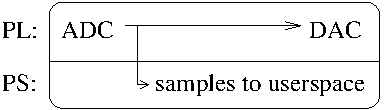
\includegraphics{objective}
\end{center}

\hspace*{-2cm}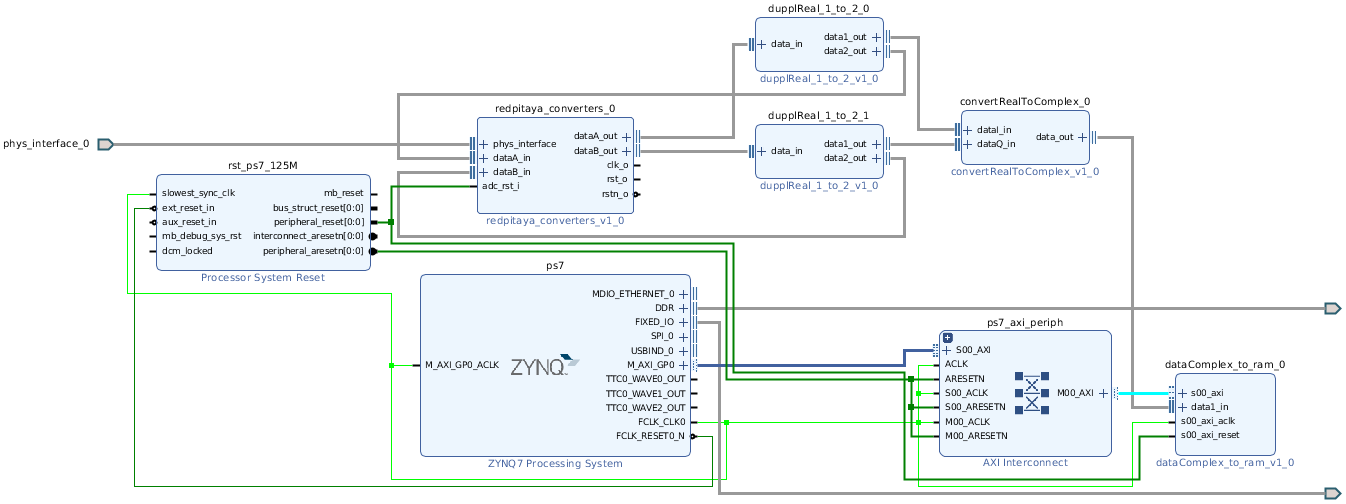
\includegraphics[width=1.2\linewidth]{combinedADC_DAC_data2ram}
\caption{Objective (top) of this tutorial and final schematic of the processing chain described
in this document.}
\label{fin}
\end{figure}

\section{Sending data to the PS: the PL side}

Transfering data towards the PS {\em in addition} to sending the stream to
the DAC requires duplicating the data on the one hand, and interleaving the two
streams from the two ADCs on the other hand.

Doing so is achieved by:
\begin{enumerate}
\item add {\tt dupplReal\_1\_to\_2}, {\tt convertRealToComplex} (converting two real
data streams to one complex) and then {\tt dataComplex\_to\_ram}
\item Double click on {\tt dupplReal\_1\_to\_2} to configure to 14 bit (or 16-bit if using
the 16-bit Redpitaya) data (doing so on the two stream doublers). Same for 
{convertRealToComplex} 
\item Link {\tt data1\_out} of each {\tt dupplReal} to {\tt data1\_in} and
{\tt data2\_in} respectively of \\{\tt convertRealToComplex}
\item Cut the wires linking the ADC and DAC, and use the two free outputs of the 
{\tt dupplReal\_1\_to\_2} blocks
\item Connect {\tt dataA\_out} and {\tt dataB\_out} of the ADCs to the two free inputs
of the {\tt dupplReal\_1\_to\_2} blocks
\item {\tt dataComplex\_to\_RAM}: configure {\tt Data Size} to 14 bits (or 16-bit if using
the 16-bit Redpitaya), {\tt Nb
Input} to 1 and 
{\tt Nb Sample} to the number of samples to be transfered.
For example, defining 4096 {\bf sample pairs} (complex numbers) each encoded as
16-bit values, or a total of 16384~bytes available to the PS.
\end{enumerate}

Once these blocks have been defined and connected, execute {\tt Run Connection 
Automation} for connecting to the AXI bus.

\section{Sending data to the PS: the Linux kernel side}

The driver needed to fetch data on the PS from Linux will be 
{\tt data\_to\_ram\_core}. Compiling this kernel module requires
exporting the variables

\begin{verbatim}
export BOARD_NAME=redpitaya
export BR_DIR=${HOME}/buildroot-2018.08.1/
\end{verbatim}

Compilation is achieved from the {\tt \$OSCIMP\_DIGITAL\_DRIVER/dataComplex\_to\_ram\_core}
directory by running \\
{\tt make install} \\
which will install the {\tt .ko} in 
{\tt \$OSCIMP\_DIGITAL\_NFS/\$BOARD\_NAME/modules}.

We have briefly introduced the {\tt devicetree overlay} in {\tt 1-PL}. In the context
of this tutorial, where we must communicate with an IP, the {\tt overlay} approach
is mandatory. This file provides both bitstream name and, through a sub-node, information
used by the Linux kernel to know which driver must be probed, and the base address of the
memory segment shared between PS and PL, allocated for communications between the IP and 
the associated driver.

%In the context of a {devicetree overlay}, we will not explictly configure
%the FPGA using the current bitstream and load the kernel module ({\tt insmod}), but will ask
%the devicetree to coherently run all the needed tasks.
The plugin to the devicetree is 
generated thanks to the {\tt module\_generator} tool located in {\tt 
\$OSCIMP\_DIGITAL\_APP/tools/module\_generator}: this tool is designed to get the definition of all
resources from an XML file written manually. In this example, the configuration file is

\lstinputlisting[language=xml]{./module_generator.xml}

%\begin{verbatim}
%<?xml version="1.0" encoding="utf-8"?>
%<drivers name="tutoriel3" version="1.0">
%    <driver name ="data16Complex_to_ram" >
%        <board_driver name="data1600" id = "0"
%            base_addr="0x43c00000" addr_size="0xffff" />
%        </driver>
%</drivers>
%\end{verbatim}

\noindent
with the {\tt name} tag including the name of the bitstream without the {\tt .bit.bin} extension
nor the ``\_wrapper'' part of its name (notice that the default name {\tt tutorial3} is given
by Vivado to generate {\tt tutorial3\_wrapper.bit.bin}). The {\tt driver} tag informs
on the kernel module to be loaded, while {\tt base\_addr} and {\tt addr\_size} provide the
address starting point and range as provided in each IP attribute by Vivado (Fig. \ref{addr}).
{\tt option} node tell {\tt module\_generator} to add {\tt DONT\_USE\_LIB} in
the Makefile. This variable is used to avoid application to be linked to the
liboscimp\_fpga (see. 4-FIR for library introduction).

\begin{figure}[h!tb]
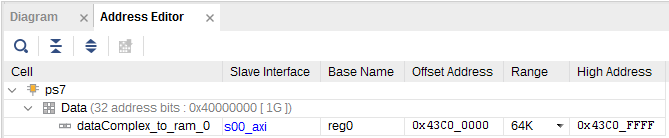
\includegraphics[width=\linewidth]{adresses}
\caption{Address range used by each IP able to communicate between the PL and PS through the AXI 
bus.}
\label{addr}
\end{figure}

This XML is used to generate devicetree file, script to load drivers and apply the overlay,
and a Makefile dedicated to compile the application, the dtbo and to install all files in
{\tt \$OSCIMP\_DIGITAL\_NFS/tutorial3}.

This task is done by this command:\\
{\tt fpga\_app/tools/module\_generator/module\_generator -dts my\_file.xml}

After generation, a new directory, called {\tt app} is present in the current
directory, containing all files. The Makefile is basic since it provides the
application name and simply includes
{\tt \$OSCIMP\_DIGITAL\_APP/Makefile.inc}. {\tt make} will compile the application
({\tt tutorial3\_us}) and the dtbo ({\tt tutorial3.dtbo}) while {\tt make install}
will 1/ create \\
{\tt \$OSCIMP\_DIGITAL\_NFS/\$BOARD\_NAME/tutorial3}, and 2/ copy binary files in
a sub-directory called {\tt bin}.

The rest needs some explanations.

\subsection{Devicetree overlay}
For the current design the overlay looks like:
\lstinputlisting{./app/tutorial3.dts}

Compared to the previous tutorials, this devicetree provides a subnode to
declare a driver. This node is describe by a name used, at runtime, for the pseudo-file
in {\tt /dev}, an attribute {\tt compatible} used by Linux to match between
this entry and the {\tt compatible} attribute of the core driver and, finally,
an attribute {\tt reg} wich provides the base address in memory and size of this slice.

\subsection{Loader script}

The second file created by {\tt module\_generator} is a script called {\tt
tutorial3\_us.sh}:

\lstinputlisting[language=bash]{./app/tutorial3_us.sh}

\noindent
this script copies the bitstream to {\tt /lib/firmware}, applies the overlay and
loads the core driver.

%and then converted to a binary {devicetree overlay} by
%
%\hspace*{-2.53cm}
%{\footnotesize
%\verb~[...]/buildroot/output/build/linux-[...]/scripts/dtc/dtc -@ -I dts -O dtb -o tutorial3.dtbo tutorial3.dts~}
%

\subsection{Source code}

This file is not provided by {\tt module\_generator} and must be created/written 
manually.

\begin{lstlisting}[language=C]
#include <stdio.h>
#include <stdint.h>
#include <fcntl.h>
#include <unistd.h>

int main()
{int k,fi,fo; char c[16384];
 fi=open("/dev/data1600",O_RDWR); fo=open("/tmp/data.bin",O_WRONLY|O_CREAT);
 for (k=1;k<5;k++) {read(fi,c,16384); write(fo,c,16384); }
 close(fi); close(fo);
}
\end{lstlisting}

\noindent
where we open {\tt /dev/data1600} to read 5 time 16384 samples and write these values in an
other file in binary format.

\section{On the Redpitaya ...}

Having completed all compilation and installation steps, we have in\\
{\tt \$OSCIMP\_DIGITAL\_NFS/\$BOARD\_NAME}:
\begin{enumerate}
\item {\tt tutorial3.dtbo}, {\tt tutorial3\_us.sh} and {\tt tutorial3\_us} in
{\tt tutorial3/bin} directory;
\item {\tt tutorial3\_wrapper.bit.bin} in {\tt tutorial3/bitstreams};
\item {\tt dataComplex\_to\_ram\_core.ko} in {\tt modules/}
\end{enumerate} 
%we are finally left with three files on the PC
%to be transfered to the embedded board (e.g. Redpitaya):
%\begin{enumerate}
%\item the {\tt .bit.bin} bitstream 
%\item the {\tt .ko} kernel module
%\item the {\tt .dtbo} devicetree overlay
%\end{enumerate}

%Having transfered these files to the embedded board, the {\em devicetree overlay} mechanism
%is activated in order to coherently load all these files by
%\begin{enumerate}
%\item {\tt cp tutorial3\_wrapper.bit.bin /lib/firmware/}
%\item {\tt mkdir /sys/kernel/config/device-tree/overlays/my\_directory}
%\item {\tt cat tutorial3.dtbo > /sys/kernel/config/device-tree/overlays/my\_directory/dtbo}
%\end{enumerate}

%Having transfered these files to the embedded board,
The next task, before using the application is to load the bitstream, the overlay and the 
driver. This is done by the command: \verb|sh tutorial3_us.sh|.

If all goes well, the blue LED on the Redpitaya board will light up (the bitstream has been
used to configure the FPGA) and the kernel module is loaded. The last step is to fetch data
from userspace: \verb|./tutorial3_us|

whos execution will generate a binary data file loaded in GNU/Octave with
\begin{lstlisting}[language=Octave]
f=fopen('data.bin')
d=fread(f,inf,'int16');
plot(d(2:2:end));
\end{lstlisting}

providing a result as exhibited in Fig. \ref{adc} in which the input of the ADC is
directly connected to the non-differential to differential amplifier input in order to
exploit aliasing on purpose (bypassing the low-pass filter).

\begin{figure}[h!tb]
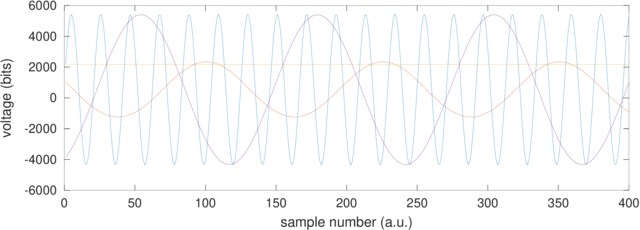
\includegraphics[width=\linewidth]{mesures}
\caption{Acquisitions from FPGA by the userspace program communicating with the kernel through
the {\tt /dev/data1600} device: sine waves the generated at a level of +6~dBm at
1~MHz, 6~MHz, 124~MHz (aliased to weaker 1~MHz) and 125~MHz (aliased to the DC signal).}
\label{adc}
\end{figure}
\end{document}
